\documentclass[10pt]{article}

\usepackage[a4paper,margin=0.65in]{geometry}
\usepackage{amsmath,amssymb}
\usepackage{graphicx}
\usepackage{booktabs}
\usepackage{array}
\usepackage{float}
\usepackage{hyperref}
\usepackage{enumitem}
\usepackage{xcolor}
\usepackage{tikz}
\usetikzlibrary{positioning,arrows.meta,shapes.geometric}

\setlist{nosep,leftmargin=*}
\renewcommand{\arraystretch}{1.2}
\setlength{\parindent}{0pt}
\setlength{\parskip}{2pt}

\tikzset{
layer/.style={
draw,
rounded corners,
minimum width=1.5cm,
minimum height=0.6cm,
align=center,
fill=blue!10,
font=\scriptsize
},
arrow/.style={
-{Latex[length=2mm]},
thin
}
}

\begin{document}

%%%%%%%%%%%%%%%%%%%%%%%%%%%%%%%%%%%%%%%%%%%%%%%%%%%%%%%%%%%%
% TITLE
%%%%%%%%%%%%%%%%%%%%%%%%%%%%%%%%%%%%%%%%%%%%%%%%%%%%%%%%%%%%

\begin{center}

{\large\textbf{Shiv Nadar University Chennai}}

\vspace{2mm}

{\normalsize\textbf{CS3807 -- Deep Learning Laboratory}}

\vspace{2mm}

{\large\textbf{Experiment 5}}

\vspace{1mm}

{\normalsize\textbf{Comprehensive Study of CNN Training, Regularization,}}

{\normalsize\textbf{Optimization, Hyperparameter Tuning, Transfer Learning}}

{\normalsize\textbf{and Cross-Validation}}
\textbf{Repository Link:}
\textbf{\url{https://github.com/Atharsh2910/Deep_Learning_Lab/tree/main/Lab5}
}

\end{center}

\vspace{3mm}

\begin{tabular}{|p{3.8cm}|p{8cm}|p{2cm}|}
\hline
Degree \& Branch & B.Tech Artificial Intelligence \& Data Science & Semester V\\ \hline
Subject Code \& Name & CS3807 -- Deep Learning Laboratory & AY: 2026--27\\ \hline
\end{tabular}

\begin{tabular}{|p{3.5cm}|p{8cm}|}
\hline
\textbf{Name} & {ATHARSH S U}\\ \hline
\textbf{Register Number} &{24011101008} \\ \hline
\textbf{Roll Number} &{24110049} \\ \hline
\textbf{Class} & {AI-DS 'A'}\\ \hline
\end{tabular}
\vspace{3mm}

%%%%%%%%%%%%%%%%%%%%%%%%%%%%%%%%%%%%%%%%%%%%%%%%%%%%%%%%%%%%
\section*{1. Objective}

The objective of this experiment is to systematically study the effect of
weight initialization, regularization, optimization algorithms, CNN
hyperparameters, transfer learning, fine-tuning and cross-validation on
image classification performance.

The experiment uses a single CNN architecture, MobileNetV2, and the
Oxford-IIIT Pet dataset. Students will analyze the effect of individual
design choices using training/validation curves and finally select a
suitable configuration using 5-fold cross-validation.

%%%%%%%%%%%%%%%%%%%%%%%%%%%%%%%%%%%%%%%%%%%%%%%%%%%%%%%%%%%%
\section*{2. Learning Outcomes}

After completing this experiment, students will be able to:

\begin{itemize}
\item explain different weight initialization strategies;
\item identify and analyze overfitting using training and validation curves;
\item compare SGD, Momentum, RMSProp and Adam;
\item explain CNN hyperparameters such as kernel size, stride, padding and pooling;
\item understand Batch Normalization and Dropout;
\item perform transfer learning and fine-tuning using MobileNetV2;
\item tune important training hyperparameters;
\item apply 5-fold cross-validation for model selection; and
\item justify the final model using accuracy, variability and computational cost.
\end{itemize}

%%%%%%%%%%%%%%%%%%%%%%%%%%%%%%%%%%%%%%%%%%%%%%%%%%%%%%%%%%%%
\section*{3. Dataset and Experimental Setup}

\textbf{Dataset: Oxford-IIIT Pet Dataset}

The Oxford-IIIT Pet Dataset contains images of cats and dogs belonging
to 37 breeds. The images are RGB and have different spatial dimensions.
For this experiment, all images are resized to

\[
224\times224\times3.
\]

The dataset is suitable for demonstrating transfer learning using
ImageNet-pretrained CNNs.

\textbf{Dataset statistics (as loaded via \texttt{tensorflow\_datasets}):}

\begin{center}
\begin{tabular}{|l|c|}
\hline
Number of classes (breeds) & 37\\
Official training examples & 3680\\
Official test examples & 3669\\
Train/validation split of the training examples & 80\% / 20\%\\
Training subset fraction actually used (GPU profile) & 60\%\\
\hline
\end{tabular}
\end{center}

The official 3680-image training split was shuffled and further divided
80/20 into an internal training set and validation set; the 20\% held
out here is used for all epoch-by-epoch validation curves in Sections
5--10. The official 3669-image test split was kept completely untouched
until the final evaluation in Section 12. Because the study trains many
models across Sections 5--11, a GPU runtime profile subsamples 60\% of
the internal training set (after the val-split) to keep total run time
reasonable while still using thousands of images per experiment.

\textbf{Experimental considerations:}

\begin{itemize}
\item Use RGB images resized to $224\times224$.
\item Normalize the input images according to the pretrained model requirements.
\item Maintain separate training, validation and test data.
\item The test set must remain untouched during hyperparameter selection.
\item Use MobileNetV2 because it is computationally lighter than many
large CNN architectures and is more suitable for CPU-based laboratory work.
\end{itemize}

%%%%%%%%%%%%%%%%%%%%%%%%%%%%%%%%%%%%%%%%%%%%%%%%%%%%%%%%%%%%
\section*{4. MobileNetV2 Architecture}

MobileNetV2 is a lightweight CNN architecture designed to reduce
computational complexity while maintaining good image representation.

Its important components include:

\begin{itemize}
\item depthwise convolution;
\item pointwise $1\times1$ convolution;
\item inverted residual blocks;
\item linear bottlenecks;
\item batch normalization; and
\item ReLU6 activation.
\end{itemize}

A simplified representation is:

\begin{center}
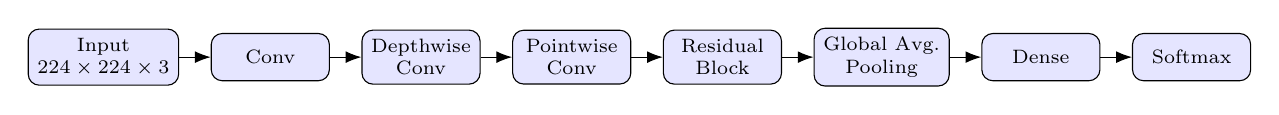
\begin{tikzpicture}[node distance=4mm]

\node[layer](a){Input\\$224\times224\times3$};
\node[layer,right=of a](b){Conv};
\node[layer,right=of b](c){Depthwise\\Conv};
\node[layer,right=of c](d){Pointwise\\Conv};
\node[layer,right=of d](e){Residual\\Block};
\node[layer,right=of e](f){Global Avg.\\Pooling};
\node[layer,right=of f](g){Dense};
\node[layer,right=of g](h){Softmax};

\foreach \x/\y in {a/b,b/c,c/d,d/e,e/f,f/g,g/h}
\draw[arrow](\x)--(\y);

\end{tikzpicture}
\end{center}

\textbf{Note:} The above diagram is a simplified conceptual representation
rather than the complete MobileNetV2 architecture.

%%%%%%%%%%%%%%%%%%%%%%%%%%%%%%%%%%%%%%%%%%%%%%%%%%%%%%%%%%%%
\section*{5. Weight Initialization}

Weight initialization determines the initial values of trainable weights
before training begins. A suitable initialization can improve convergence
and reduce problems such as vanishing or exploding activations.

Students should investigate:

\begin{itemize}
\item Zero initialization
\item Random initialization
\item Xavier/Glorot initialization
\item He initialization
\end{itemize}

\subsection*{Expected Analysis}

Students should compare the initialization strategies using:

\textbf{Plot 1: Training Loss vs. Epoch}

\begin{itemize}
\item X-axis: Epoch
\item Y-axis: Training Loss
\item Plot one curve for each initialization method.
\end{itemize}

\textbf{Plot 2: Validation Accuracy vs. Epoch}

\begin{itemize}
\item X-axis: Epoch
\item Y-axis: Validation Accuracy (\%)
\item Plot one curve for each initialization method.
\end{itemize}

Students should identify which initialization gives faster and more
stable convergence.

\begin{figure}[H]
\centering
\includegraphics[width=0.72\textwidth]{images/plot1_init_loss.png}
\end{figure}

\begin{figure}[H]
\centering
\includegraphics[width=0.72\textwidth]{images/plot2_init_valacc.png}
\end{figure}

\textbf{Observed Results (10 epochs, MobileNetV2 head, Adam, lr $=10^{-3}$):}

\begin{center}
\begin{tabular}{|l|c|c|}
\hline
Initialization & Final Training Loss & Best Validation Accuracy (\%)\\
\hline
Zero & 3.6105 & 2.85\\
Random Normal & 0.1464 & 98.37\\
Xavier/Glorot & 0.1286 & 99.05\\
He & 0.1389 & 98.91\\
\hline
\end{tabular}
\end{center}



%%%%%%%%%%%%%%%%%%%%%%%%%%%%%%%%%%%%%%%%%%%%%%%%%%%%%%%%%%%%
\section*{6. Regularization and Overfitting}

Overfitting occurs when a model performs very well on the training data
but generalizes poorly to unseen data.

Students should compare:

\begin{itemize}
\item No regularization
\item L2 regularization
\item Dropout
\item Batch Normalization
\end{itemize}

\subsection*{Expected Plots}

\textbf{Plot 3: Training and Validation Accuracy vs. Epoch}

\begin{itemize}
\item X-axis: Epoch
\item Y-axis: Accuracy (\%)
\item Plot separate curves for training and validation accuracy.
\end{itemize}

Students should identify the generalization gap.

\textbf{Plot 4: Training and Validation Loss vs. Epoch}

\begin{itemize}
\item X-axis: Epoch
\item Y-axis: Loss
\item Plot training and validation loss.
\end{itemize}

Students should identify whether validation loss begins to increase while
training loss continues to decrease.

\begin{figure}[H]
\centering
\includegraphics[width=0.95\textwidth]{images/plot3_reg_acc.png}
\end{figure}

\begin{figure}[H]
\centering
\includegraphics[width=0.95\textwidth]{images/plot4_reg_loss.png}
\end{figure}

\textbf{Final-epoch generalization gap (Train Accuracy $-$ Validation Accuracy):}

\begin{center}
\begin{tabular}{|l|c|}
\hline
Configuration & Gap (percentage points)\\
\hline
No Regularization & $+0.17$\\
L2 Regularization & $-0.45$\\
Dropout & $-4.92$\\
Batch Normalization & $-1.34$\\
\hline
\end{tabular}
\end{center}

%%%%%%%%%%%%%%%%%%%%%%%%%%%%%%%%%%%%%%%%%%%%%%%%%%%%%%%%%%%%
\section*{7. Batch Normalization}

Batch Normalization normalizes activations within a mini-batch during
training.

For a mini-batch

\[
x_1,x_2,\ldots,x_m,
\]

the batch mean is

\[
\mu_B=\frac{1}{m}\sum_{i=1}^{m}x_i
\]

and the batch variance is

\[
\sigma_B^2=
\frac{1}{m}\sum_{i=1}^{m}(x_i-\mu_B)^2.
\]

The normalized activation is

\[
\hat{x}_i=
\frac{x_i-\mu_B}
{\sqrt{\sigma_B^2+\epsilon}}.
\]

The final output is

\[
y_i=\gamma\hat{x}_i+\beta,
\]

where $\gamma$ and $\beta$ are learnable parameters.

\subsection*{Numerical Example}

Consider

\[
x=[2,4,6,8].
\]

The mean is

\[
\mu_B=\frac{2+4+6+8}{4}=5.
\]

The variance is

\[
\sigma_B^2=
\frac{(2-5)^2+(4-5)^2+(6-5)^2+(8-5)^2}{4}
=5.
\]

Therefore,

\[
\sqrt{5}\approx2.236.
\]

Ignoring the very small $\epsilon$,

\[
\hat{x}_1=\frac{2-5}{2.236}\approx-1.342,
\]

\[
\hat{x}_2=\frac{4-5}{2.236}\approx-0.447,
\]

\[
\hat{x}_3=\frac{6-5}{2.236}\approx0.447,
\]

\[
\hat{x}_4=\frac{8-5}{2.236}\approx1.342.
\]

Hence,

\[
\boxed{
\hat{x}\approx[-1.342,-0.447,0.447,1.342]
}
\]

If $\gamma=1$ and $\beta=0$, these are the final outputs.

\textbf{Inference:} Batch Normalization produces approximately
zero-centred and unit-scaled activations for this mini-batch. The
learnable $\gamma$ and $\beta$ allow the network to learn an appropriate
scale and shift.

\textbf{Plot 5: With vs. Without Batch Normalization}

\begin{itemize}
\item X-axis: Epoch
\item Y-axis: Validation Accuracy (\%)
\item Compare two curves: With BN and Without BN.
\end{itemize}

\begin{figure}[H]
\centering
\includegraphics[width=0.72\textwidth]{images/plot5_bn.png}
\end{figure}


%%%%%%%%%%%%%%%%%%%%%%%%%%%%%%%%%%%%%%%%%%%%%%%%%%%%%%%%%%%%
\section*{8. Optimization Algorithms}

Students should compare the following optimization methods:

\begin{itemize}
\item SGD
\item Momentum
\item RMSProp
\item Adam
\end{itemize}

The objective is to study convergence speed, stability and final
validation performance.

\textbf{Plot 6: Training Loss vs. Epoch for Different Optimizers}

\begin{itemize}
\item X-axis: Epoch
\item Y-axis: Training Loss
\item One curve for each optimizer.
\end{itemize}

\textbf{Plot 7: Validation Accuracy vs. Epoch for Different Optimizers}

\begin{itemize}
\item X-axis: Epoch
\item Y-axis: Validation Accuracy (\%)
\item One curve for each optimizer.
\end{itemize}

\begin{figure}[H]
\centering
\includegraphics[width=0.72\textwidth]{images/plot6_opt_loss.png}
\end{figure}

\begin{figure}[H]
\centering
\includegraphics[width=0.72\textwidth]{images/plot7_opt_valacc.png}
\end{figure}

\begin{center}
\begin{tabular}{|l|c|c|c|c|}
\hline
Optimizer & Final Loss & Best Val. Accuracy & Epoch to Converge & Time\\
\hline
SGD & 2.1269 & 61.55\% & 10 & 116.3 s\\
Momentum & 0.4236 & 93.61\% & 9 & 114.2 s\\
RMSProp & 0.1251 & 98.51\% & 10 & 113.9 s\\
Adam & 0.1350 & 99.05\% & 9 & 115.3 s\\
\hline
\end{tabular}
\end{center}


%%%%%%%%%%%%%%%%%%%%%%%%%%%%%%%%%%%%%%%%%%%%%%%%%%%%%%%%%%%%
\section*{9. CNN Hyperparameter Tuning}

The following hyperparameters should be investigated:

\begin{center}
\begin{tabular}{|l|l|}
\hline
Hyperparameter & Suggested Values\\
\hline
Learning Rate & $0.001,\;0.0001$\\
Batch Size & 16, 32, 64\\
Dropout Rate & 0, 0.25, 0.5\\
Optimizer & SGD, Adam\\
Fine-Tuning Learning Rate & $10^{-4},10^{-5}$\\
Frozen Layers & Frozen base / Partial unfreezing\\
\hline
\end{tabular}
\end{center}

For CNN concepts, students should also understand:

\begin{itemize}
\item kernel/filter;
\item stride;
\item padding;
\item pooling;
\item number of channels; and
\item depthwise separable convolution.
\end{itemize}

For a convolution operation, the output dimension can be calculated as

\[
O=
\left\lfloor
\frac{N+2P-K}{S}
\right\rfloor+1,
\]

where $N$ is input size, $K$ is kernel size, $P$ is padding and $S$ is
stride.

\textbf{Numerical check:} For $N=224$, $K=3$, $P=1$, $S=1$ (a
``same''-padded $3\times3$ convolution), $O=224$, i.e.\ the spatial size
is preserved. For $N=224$, $K=3$, $P=0$, $S=2$ (a typical MobileNetV2
stem convolution), $O=\left\lfloor\frac{224-3}{2}\right\rfloor+1=111$.

\textbf{Experimental rule:} During a controlled hyperparameter study,
change one hyperparameter at a time while keeping the remaining settings
fixed.

\textbf{Plot 8: Learning Rate vs. Validation Accuracy}

\begin{itemize}
\item X-axis: Learning Rate
\item Y-axis: Validation Accuracy (\%)
\end{itemize}

\begin{figure}[H]
\centering
\includegraphics[width=0.6\textwidth]{images/plot8_lr.png}
\end{figure}

\begin{center}
\begin{tabular}{|l|c|}
\hline
Learning Rate & Best Validation Accuracy (\%)\\
\hline
$10^{-3}$ & 97.69\\
$10^{-4}$ & 89.13\\
\hline
\end{tabular}
\end{center}


\textbf{Plot 9: Batch Size vs. Validation Accuracy}

\begin{itemize}
\item X-axis: Batch Size
\item Y-axis: Validation Accuracy (\%)
\end{itemize}

\begin{figure}[H]
\centering
\includegraphics[width=0.6\textwidth]{images/plot9_batchsize.png}
\end{figure}

\begin{center}
\begin{tabular}{|l|c|}
\hline
Batch Size & Best Validation Accuracy (\%)\\
\hline
16 & 98.23\\
32 & 98.78\\
64 & 98.51\\
\hline
\end{tabular}
\end{center}


\textbf{Plot 10: Dropout Rate vs. Validation Accuracy}

\begin{itemize}
\item X-axis: Dropout Rate
\item Y-axis: Validation Accuracy (\%)
\end{itemize}

\begin{figure}[H]
\centering
\includegraphics[width=0.6\textwidth]{images/plot10_dropout.png}
\end{figure}

\begin{center}
\begin{tabular}{|l|c|}
\hline
Dropout Rate & Best Validation Accuracy (\%)\\
\hline
0.00 & 99.05\\
0.25 & 97.69\\
0.50 & 97.55\\
\hline
\end{tabular}
\end{center}


%%%%%%%%%%%%%%%%%%%%%%%%%%%%%%%%%%%%%%%%%%%%%%%%%%%%%%%%%%%%
\section*{10. Transfer Learning and Fine-Tuning}

MobileNetV2 pretrained on ImageNet should be used.

\subsection*{Case A: Feature Extraction}

\[
\text{Pretrained MobileNetV2}
\rightarrow
\text{Freeze Base}
\rightarrow
\text{New Classifier}
\]

The pretrained convolutional layers are frozen and only the newly added
classification layers are trained.

\subsection*{Case B: Fine-Tuning}

\[
\text{Pretrained MobileNetV2}
\rightarrow
\text{Unfreeze Selected Layers}
\rightarrow
\text{Small Learning Rate}
\]

The upper layers of the pretrained network are unfrozen and trained with
a smaller learning rate.

\textbf{Plot 11: Feature Extraction vs. Fine-Tuning}

\begin{itemize}
\item X-axis: Epoch
\item Y-axis: Validation Accuracy (\%)
\item Two curves: Feature Extraction and Fine-Tuning.
\end{itemize}

\begin{figure}[H]
\centering
\includegraphics[width=0.72\textwidth]{images/plot11_fe_vs_ft.png}
\end{figure}


\textbf{Plot 12: Training and Validation Loss}

Students should compare the loss curves before and after fine-tuning.

\begin{figure}[H]
\centering
\includegraphics[width=0.72\textwidth]{images/plot12_loss_ft.png}
\end{figure}

\textbf{Discussion:} Explain why fine-tuning normally requires a smaller
learning rate than training a newly initialized classifier.

Because the unfrozen base layers already hold well-optimized
ImageNet-pretrained weights, a large learning rate would apply large
gradient updates that quickly destroy this useful representation
(``catastrophic forgetting''). A small learning rate ($10^{-5}$ here,
versus $10^{-3}$ for the freshly initialized head) allows the pretrained
weights to be adjusted only slightly, adapting them to the new dataset
while preserving the general visual features already learned.

\textbf{Fine-tuning hyperparameter sweep (8 epochs each):}

\begin{center}
\begin{tabular}{|l|c|}
\hline
Fine-Tuning Learning Rate (70\% frozen) & Best Validation Accuracy (\%)\\
\hline
$10^{-4}$ & 95.38\\
$10^{-5}$ & 64.40\\
\hline
\end{tabular}
\end{center}

\begin{center}
\begin{tabular}{|l|c|}
\hline
Frozen-Layer Strategy (lr fixed) & Best Validation Accuracy (\%)\\
\hline
Frozen base (feature extraction), lr $=10^{-3}$ & 98.64\\
Partial unfreeze (top 30\%), lr $=10^{-5}$ & 64.81\\
\hline
\end{tabular}
\end{center}


%%%%%%%%%%%%%%%%%%%%%%%%%%%%%%%%%%%%%%%%%%%%%%%%%%%%%%%%%%%%
\section*{11. K-Fold Cross-Validation}

After the individual studies, select 3--4 promising configurations.

Use 5-fold cross-validation on the training data.

For $K=5$,

\[
\bar{A}=
\frac{1}{5}\sum_{i=1}^{5}A_i
\]

and

\[
SD=
\sqrt{
\frac{1}{5}
\sum_{i=1}^{5}(A_i-\bar{A})^2
}.
\]

Report the result as

\[
\boxed{\bar{A}\pm SD}.
\]

The independent test set must not be used during hyperparameter selection.

Four shortlisted configurations, all built on MobileNetV2 with a
GlobalAveragePooling $\to$ BatchNorm $\to$ Dense(128) $\to$ Dropout $\to$
Softmax head, were evaluated:
\textbf{C1 Baseline} (Glorot init, dropout 0.3, Adam lr $10^{-3}$);
\textbf{C2 Best-Init/He} (He init, dropout 0.3, Adam lr $10^{-3}$);
\textbf{C3 Dropout 0.5} (He init, dropout 0.5, Adam lr $10^{-3}$); and
\textbf{C4 Lower LR} (He init, dropout 0.3, Adam lr $10^{-4}$).

\begin{center}
\begin{tabular}{|l|c|c|c|c|c|c|}
\hline
Configuration & F1 & F2 & F3 & F4 & F5 & Mean $\pm$ SD\\
\hline
C1 (Baseline) & 89.83 & 93.48 & 87.82 & 88.39 & 88.95 & $89.69\pm2.01$\\
C2 (Best Init -- He) & 90.68 & 93.77 & 87.25 & 89.24 & 89.52 & $90.09\pm2.14$\\
C3 (Dropout 0.5) & 88.98 & 94.33 & 86.69 & 88.10 & 89.80 & $89.58\pm2.59$\\
C4 (Lower LR) & 82.77 & 82.72 & 81.59 & 79.60 & 82.44 & $81.82\pm1.19$\\
\hline
\end{tabular}
\end{center}

\textbf{Plot 13: 5-Fold Cross-Validation Accuracy}

\begin{itemize}
\item X-axis: Hyperparameter Configuration
\item Y-axis: Mean Validation Accuracy (\%)
\item Include standard-deviation error bars.
\end{itemize}

\begin{figure}[H]
\centering
\includegraphics[width=0.72\textwidth]{images/plot13_cv.png}
\end{figure}

Students should discuss both mean performance and variability.

%%%%%%%%%%%%%%%%%%%%%%%%%%%%%%%%%%%%%%%%%%%%%%%%%%%%%%%%%%%%
\section*{12. Final Model Evaluation}

After selecting the best configuration using cross-validation:

\begin{enumerate}
\item Retrain the selected configuration using the complete training data.
\item Keep the independent test set untouched until this stage.
\item Evaluate the final model on the test set.
\end{enumerate}

The best configuration selected by cross-validation, C2\_BestInit\_HeNorm
(He initialization, dropout 0.3, BatchNorm, Adam lr $10^{-3}$), was
retrained on the complete training split (18 epochs) and evaluated once
on the untouched test set.

Report:

\begin{center}
\begin{tabular}{|l|c|}
\hline
Metric & Value\\
\hline
Mean CV Accuracy & 90.09\%\\
CV Standard Deviation & 2.14\\
Test Accuracy & 89.21\%\\
Precision (weighted) & 0.8948\\
Recall (weighted) & 0.8921\\
F1-score (weighted) & 0.8909\\
Training Time & 181.9 s\\
Number of Parameters & 2{,}431{,}845\\
\hline
\end{tabular}
\end{center}

\textbf{Plot 14: Confusion Matrix}

Students should identify:

\begin{itemize}
\item the best classified classes;
\item the most frequently confused classes; and
\item possible visual reasons for misclassification.
\end{itemize}

\begin{figure}[H]
\centering
\includegraphics[width=0.85\textwidth]{images/plot14_confmat.png}
\end{figure}

\textbf{Best classified classes (per-class accuracy):} Yorkshire Terrier
(100.0\%), Samoyed (100.0\%), Japanese Chin (99.0\%), Shiba Inu (99.0\%)
and Leonberger (99.0\%).

\textbf{Most confused classes (lowest per-class accuracy):} American
Pit Bull Terrier (51.0\%), Ragdoll (69.0\%), British Shorthair (71.0\%),
Staffordshire Bull Terrier (74.2\%) and Birman (76.0\%).


\textbf{Optional Plot 15: Misclassified Images}

Display representative incorrectly classified images and provide a
brief explanation for each.

\begin{figure}[H]
\centering
\includegraphics[width=0.85\textwidth]{images/plot15_misclassified.png}
\end{figure}


%%%%%%%%%%%%%%%%%%%%%%%%%%%%%%%%%%%%%%%%%%%%%%%%%%%%%%%%%%%%
\section*{13. Overall Results}

\begin{center}
\begin{tabular}{|l|c|c|c|c|}
\hline
Configuration & CV Accuracy & SD & Test/Val. Accuracy & Training Time\\
\hline
Baseline & -- & -- & 88.85\% & 153.4 s\\
Best Initialization (He) & -- & -- & 98.91\% & --\\
Best Regularization (Dropout) & -- & -- & 97.01\% & --\\
Best Optimizer (Adam) & -- & -- & 99.05\% & 115.3 s\\
Best Hyperparameters (C2\_BestInit\_HeNorm) & 90.09\% & 2.14 & -- & --\\
Fine-Tuned Model & -- & -- & 99.73\% & --\\
\textbf{FINAL MODEL (retrained + tested)} & \textbf{90.09\%} & \textbf{2.14} & \textbf{89.21\%} & \textbf{181.9 s}\\
\hline
\end{tabular}
\end{center}


\begin{figure}[H]
\centering
\includegraphics[width=0.78\textwidth]{images/plot16_overall_comparison.png}
\end{figure}



%%%%%%%%%%%%%%%%%%%%%%%%%%%%%%%%%%%%%%%%%%%%%%%%%%%%%%%%%%%%
\section*{14. Required Inference for Plots}

For every major plot, students must write a short inference containing:

\begin{enumerate}
\item What does the plot show?
\item What trend is observed?
\item Why might the observed trend occur?
\end{enumerate}

Each inference should be approximately 2--3 lines.

%%%%%%%%%%%%%%%%%%%%%%%%%%%%%%%%%%%%%%%%%%%%%%%%%%%%%%%%%%%%
\section*{15. Discussion Questions}

\begin{enumerate}

\item \textbf{What is the difference between model parameters and hyperparameters?}\\
Parameters are values that are learned automatically from
data during training, Eg., Weights, bias, etc. Hyperparameters are manually set before training. Eg., LR, epochs, droupout etc.

\item \textbf{Why is weight initialization important?}\\
Weight initialization is important because it affects the rate of convergence. High initializations can cause to overshoot the minima and may lead to exploding gradients whereas low initializations may cause slower convergence and vanishing gradients. Thus initialization in important in gradient descent.

\item \textbf{Why can zero initialization be problematic for neural networks?}\\
Zero initialization leads to a situation where every neuron gives the same output and during backpropagation it receives the same gradient. Thus all the neurons remain identical.

\item \textbf{Compare Xavier and He initialization.}\\
Xavier initialization scales weights based on the number of input and output units of a layer and is derived assuming a linear or tanh/sigmoid activation. He initialization scales weights using only the number of input units, with a larger variance suited to ReLU activations.

\item \textbf{How can training and validation curves be used to identify overfitting?}\\
If the training loss and validation loss varies significantly in the curve. The training error reduces significantly wheread the validation error remains high above.

\item \textbf{How does Dropout reduce overfitting?}\\
During training, Dropout randomly deactivates a fraction of neurons in a layer on each forward pass. This reduces the dependency on a particular neuron and reduces memorization. Thereby this prevents overfitting by minimizing the possibilities of memorization.

\item \textbf{What is the purpose of Batch Normalization?}\\
Batch normalization divides the network into multiple batches and normalizes the batch's mean to zero and standard deviation to 1. This reduces the internal covariance shift and speeds the convergence.

\item \textbf{Explain the numerical Batch Normalization example.}\\
For the mini-batch $x=[2,4,6,8]$: the mean is
$\mu_B=(2+4+6+8)/4=5$; the variance is
$\sigma_B^2=\frac{(2-5)^2+(4-5)^2+(6-5)^2+(8-5)^2}{4}=5$, so
$\sqrt{\sigma_B^2}\approx2.236$. Normalizing each value gives
$\hat{x}\approx[-1.342,-0.447,0.447,1.342]$, which has (approximately)
zero mean and unit variance. With $\gamma=1,\beta=0$ the output $y$
equals $\hat{x}$ exactly.

\item \textbf{What are the roles of $\gamma$ and $\beta$?}\\
$\gamma$ and $\beta$ are learnable parameters applied after normalization. They let the network undo or adjust the fixed zero-mean/unit-variance normalization if that is not optimal for a given layer,.

\item \textbf{Compare SGD, Momentum, RMSProp and Adam.}\\
SGD uses random gradient descent where the gradients are updated in random order. This causes noise and may slower the convergence. Momentum based GD, accumulates the exponential moving average of past gradients, thereby damping oscillation and speeding up convergence. RMS prop uses the moving average of squared gradients and ADAM is the combination of Momentum and RMS Prop, thereby converging faster.

\item \textbf{What happens when the learning rate is too large?}\\
A higher learning rate may lead to Exploding gradient and the may lead to overshooting of minima. This could lead to oscillations and model may fail to converge at all.

\item \textbf{What happens when the learning rate is too small?}\\
If the learning rate is too low, they convergence slowers. It requires more number of epochs to reach the solution.

\item \textbf{What is the effect of increasing batch size?}\\
Increasing the batch size may lead to smoother and lower variance of gradients per step. This may also lead to fewer updation per epoch but will improve the validation accuracy by better generalization.

\item \textbf{Explain stride and padding.}\\
Stride is the step size  by which the convolution kernel
moves across the input. Padding adds extra border pixels  around the input so that the kernel can be applied to the edges.

\item \textbf{Why is MobileNetV2 computationally efficient?}\\
MobileNetV2 replaces standard convolutions with depthwise separable convolutions, which  reduces the number of operations and parameters compared to a standard
convolution with the same receptive field. It further uses inverted residual blocks with linear bottlenecks to keep low-dimensional representations compact while still allowing rich, expanded intermediate features.

\item \textbf{What is depthwise separable convolution?}\\
It factorizes a standard convolution into two steps, a depthwise convolution, which applies a single spatial filter independently to each input channel, and a pointwise $1\times1$ convolution, which combines the depthwise outputs across channels.

\item \textbf{What is transfer learning?}\\
Transfer learning reuses a model or a pre trained features on general dataset as the starting point for a new, related task rather than training a model from randomly initialized weights on the target dataset alone.

\item \textbf{Differentiate feature extraction and fine-tuning.}\\
In feature extraction, the pretrained convolutional
base is frozen entirely and only a new classification head is trained on top of its fixed features. In fine-tuning, some of the upper base layers are unfrozen and trained jointly with the head, using a much smaller learning rate, allowing the pretrained features to adapt to the new task.

A smaller learning rate allows adaptation of the older trained weights to the new dataset with forgetting what was learned earlier, allowing faster convergence.

\item \textbf{Why is K-Fold Cross-Validation useful for hyperparameter selection?}\\
K-Fold cross validation trains and evaluates the dataest on K different splits of the same data. This reduces overfitting and improves generalisation.

\item \textbf{Why must the test set remain untouched during tuning?}\\
The test set must remain unseen during training so as to ensure that the model remains effective in its estimation. Exposing the test data might make the model learn the test set and does not give a proper evaluation on an unseen set.

\item \textbf{Why should mean and standard deviation both be reported?}\\
Mean measures the central tendency or the performance of the model whereas the standard deviation reports how consistent is model performing across all runs.

\item \textbf{Is the highest validation accuracy always sufficient to select a model?}\\
No, a highest validation accuracy is not always sufficient to select a model, as high accuracy in a single split might not be the same across splits/folds. It does not give the true picture of performance across all splits.
\end{enumerate}

%%%%%%%%%%%%%%%%%%%%%%%%%%%%%%%%%%%%%%%%%%%%%%%%%%%%%%%%%%%%
\section*{16. Additional Exercise}

Select two new combinations of learning rate, dropout, batch size and
fine-tuning strategy. Evaluate them using 5-fold cross-validation and
compare their results with the selected configuration.

Students must justify whether the new configuration is preferable based
on accuracy, standard deviation, computational cost and final test
performance.

%%%%%%%%%%%%%%%%%%%%%%%%%%%%%%%%%%%%%%%%%%%%%%%%%%%%%%%%%%%%
\section*{17. Expected Outcome}

Students should experimentally demonstrate that CNN performance is
strongly influenced by initialization, regularization, optimization and
hyperparameter choices. They should understand the MobileNetV2 architecture,
perform transfer learning and fine-tuning, and select a reliable final
configuration using 5-fold cross-validation.

%%%%%%%%%%%%%%%%%%%%%%%%%%%%%%%%%%%%%%%%%%%%%%%%%%%%%%%%%%%%
\section*{18. References}

\begin{enumerate}
\item Ian Goodfellow, Yoshua Bengio and Aaron Courville,
\emph{Deep Learning}, MIT Press, 2016.

\item Sergey Ioffe and Christian Szegedy,
``Batch Normalization: Accelerating Deep Network Training by Reducing
Internal Covariate Shift,'' ICML, 2015.

\item Mark Sandler, Andrew Howard, Menglong Zhu, Andrey Zhmoginov and
Liang-Chieh Chen, ``MobileNetV2: Inverted Residuals and Linear
Bottlenecks,'' CVPR, 2018.

\item Omkar M. Parkhi, Andrea Vedaldi, Andrew Zisserman and C. V. Jawahar,
``Cats and Dogs,'' IEEE Conference on Computer Vision and Pattern
Recognition, 2012.

\item TensorFlow Documentation:
\url{https://www.tensorflow.org}

\item Keras Documentation:
\url{https://keras.io}
\end{enumerate}

\end{document}
